\documentclass[a4paper,12pt]{article}
\usepackage[utf8x]{inputenc}
\usepackage[ukrainian]{babel}
\usepackage{listings}
\lstset{language=Python}
\usepackage{graphicx}
\usepackage{fixltx2e} %text sub- and superscripts
\pagestyle{plain}
\frenchspacing
\usepackage{icomma} % коскі ў матэматычным рэжыме
\usepackage{indentfirst} %Першы абзац з водступам
\renewcommand{\arraystretch}{2} %Іначай формулы ў матрыцы зліпаюцца з лініямі
\usepackage{array}
\usepackage{longtable}

% To be edited when needed %%%%%%%%%%
\newcommand{\progname}{\textit} % Стыль адлюстравання імёнаў праграм
\newcommand{\aknowl}{\textit} % Стыль для падзяк
%%%%%%%%%%%%%%%%%%%%%%%%%%%%%%%%%%%%%

\begin{document}

\renewcommand{\figurename}{Рыс.} % Не перакідаць у прэамбулу --- не працуе, чаму -- халера ведае.
\renewcommand{\abstractname}{Анатацыя}
\renewcommand{\refname}{Літаратура}

\title{ШЛЯХІ АКСЕЛЕРАЦЫІ ВЫКАНАННЯ ВЫЛІЧАЛЬНАЙ НАГРУЗКІ НА PYTHON}
\author{Літвіненка А.С.\\tenebrosus.scriptor@gmail.com\\Кіеўскі нацыянальны ўніверсітэт імя Тараса Шаўчэнкі}
\date{}
\maketitle

\begin{abstract}
Interpreted programming languages are known for their flexibility and convenience, but suffer from low execution speed comparing to compiled ones. However, they find a use for time-consuming applications. The enhanced methods of acceleration for interpreted languages are available, first of all just-in-time (JIT) compilation. The effect of the JIT compilation on the execution speed of a time-consuming scientific program is reported, and a few implementations of JIT compilers for Python are compared. \progname{PyPy} was found to be the fastest one, \progname{Psyco} --- slightly slower, \progname{Unladen Swallow} --- nearly useless.
\end{abstract}

Інтэрпрэтаваныя мовы праграмавання ўсё часцей ужываюцца пры напісанні ПЗ для разнастайных сфераў застасавання, ў тым ліку такіх, што традыцыйна не асацыююцца з інтэрпрэтаванымі мовамі, а менавіта --- напісанне ПЗ, якое патрабуе вялікіх вылічальных рэсурсаў.

Так, напрыклад, існуе напісаная часткова на Python бібліятэка для квантавахімічнага мадэліравання \progname{pDynamo} \cite{pDynamo}, аўтары якой адмовіліся ад традыцыйнага ў гэтай галіне выбару між Fortran, C або C++ і сваіх ранейшых напрацовак на Fortran, і аддалі перавагу інтэрфейсу на Python (з рэалізацыяй найбольш крытычнай да хуткасці часткі коду на C). Прычыны поспехаў інтэрпрэтаваных моваў у гэтай галіне ў выпадку навуковых праграм, верагодна, абумоўленыя лёгкасцю распрацоўкі для неадмыслоўцаў.

Таксама гэтыя мовы зручней для распрацоўкі з элементамі рэфлектыўнага праграмавання (а менавіта, калі праграме неабходна генераваць частку ўласнага коду).

Аўтарам дакладу была распрацавана праграма \progname{Mj{\"o}llnir}, якая выконвае інтэрпрэтацыю вынікаў магнетахімічнага эксперыменту з выкарыстаннем паўнаматрычнага метаду рашэння аператарных ураўненняў для спін-гамільтаніяна магнітных узаемадзеянняў, зыходзячы з мадэлі, якая задаецца карыстальнікам \cite{Mjollnir}. Для рашэння гэтае задачы неабходна на падставе мадэлі пабудаваць матрыцы спін-гамільтаніяна (прыклад на рыс.~\ref{fig:spin_ham}), прычым у алгебраічным (сімвальным) выглядзе. Алгарытм пабудовы быў рэалізаваны на Python. Праграму можна атрымаць ад аўтара пад варункамі ліцэнзіі GNU GPL v3.

Безумоўна, праблема хуткасці выканання ў такім выпадку стаецца актуальнай.


\begin{figure}[ht]
$$
\left(
\begin{array}{c|cccc}
\mathit{z}&|+\frac{1}{2};+\frac{1}{2}\rangle&|+\frac{1}{2};-\frac{1}{2}\rangle&|-\frac{1}{2};+\frac{1}{2}\rangle&|-\frac{1}{2};-\frac{1}{2}\rangle\\
\hline
\langle+\frac{1}{2};+\frac{1}{2}|&\mu H_zg_z-\frac{1}{2}J_z&0&0&0\\
\langle+\frac{1}{2};-\frac{1}{2}|&0&\frac{1}{2}J_z&-J_z&0\\
\langle-\frac{1}{2};+\frac{1}{2}|&0&-J_z&\frac{1}{2}J_z&0\\
\langle-\frac{1}{2};-\frac{1}{2}|&0&0&0&-\mu H_zg_z-\frac{1}{2}J_z\\
\end{array}
\right)
$$
\caption{Матрыца спін-гамільтаніяна для асі \textit{z} для комплексу Cu\textsubscript{2}.}
\label{fig:spin_ham}
\end{figure}

Метады акселерацыі выканання прадугледжваюць адыход ад чыстай інтэрпрэтацыі зыходнага коду ў момант выканання і пераход да разнастайных гібрыдных схемаў трансляцыі.

Па-першае, самая крытычная да рэсурсаў частка функцыянальнасці можа быць напісана на кампіляванай мове праграмавання. Але такі падыход патрабуе перапісвання коду і можа ўскладняць рэалізацыю.

Ускосным застасаваннем такога падыходу з'яўляецца выкарыстанне адных канструкцый мовы замест іншых, аналагічных, але хутчэйшых\cite{Optimize}.  Так, сапраўды, інструкцыя:
\begin{lstlisting}
    map(operator.add, l1, l2) 
\end{lstlisting}
хутчэй, чым:
\begin{lstlisting}
    map(lambda x,y: x+y, l1, l2)
\end{lstlisting}
 А спроба сабраць матрыцу ў адзін радок інструкцыяй:
\begin{lstlisting}
    collect_str+=a[i][j]  
\end{lstlisting}
 у цыкле істотна праграе інструкцыі:
\begin{lstlisting} 
    "".join(map(lambda x:"".join(x),a)).
\end{lstlisting}
У той жа час, неабходна дакладна ведаць спосабы рэалізацыі тых ці іншых інструкцый (якія могуць змяняцца з часам і залежаць ад рэалізацыі).

Прэкампіляцыя ў байт-код з'яўляецца традыцыйнай і выкарыстоўваецца заўсёды, калі ёсць такая мажлівасць.

Існуюць праэкты статычных кампілятараў падмноства мовы Python у машынны код, напрыклад, \progname{Shedskin}. Праэкт \progname{PyPy}, акрамя іншых застасаванняў, здольны статычна кампіляваць г.зв. падмноства RPython. На жаль, гэты падыход абмяжоўвае мажлівасці мовы (у прыватнасці, яго складана застасаваць для ўжо гатовага коду).

Найбольш цікавымі з'яўляюцца праэкты JIT-кампілятараў:
\begin{itemize}
\item Модуль \progname{Psyco}. Рэалізаваны як модуль \progname{CPython} (стандартнае рэалізацыі мовы). З'яўляецца найбольш старым, вядомым, зручным, а да апошняга часу --- і самым хуткім. Недахопы: прывязаны да версіі інтэрпрэтатара і платформы (толькі x86), прычым распрацоўка новых версій ускладненая (напрыклад, версіі пад Python 2.7 няма дагэтуль).

\item Праэкт \progname{PyPy}. З'яўляецца інтэпрэтатарам і JIT-кампілятарам. Хуткасць выканання расце ад версіі да версіі і ўжо перавышае хуткасць Psyco \cite{speed}. Ускладненая праца з вонкавымі бібліятэкамі на C.

\item Праэкт \progname{Unladen Swallow}. Пазіцыянуецца як аптымізаваны \progname{CPython} з JIT-кампіляцыяй. Пакуль што працуе нашмат павольней папярэдніх двух.
\end{itemize}

Агульная праблема усіх JIT-рэалізацый --- патрабаванне большага аб'ёму памяці, чым \progname{CPython}.
Вынікі сінтэтычных тэстаў хуткасці наяўныя ў Сеціве \cite{speed}. Для праверкі эфекту акселерацыі ў выпадку праграмы \progname{Mj{\"o}llnir} былі выкананыя тэсты для біядзернага комплексу медзі (Cu\textsubscript{2}, 4 базісныя функцыі), трыядзернага Fe\textsubscript{2}Co (432) і 4-ядзернага Mn\textsubscript{4} (625). Усярэдненыя вынікі для 10 запускаў (Core 2 Duo 2.4 GHz, Linux Fedora 12) прадстаўленыя на рыс.~\ref{pic:benchmark} і ў табл.~\ref{tab:benchmark}, давяральныя інтэрвалы былі разлічаныя паводле размеркавання Ст'юдэнта.

\begin{figure}[ht]
\centering{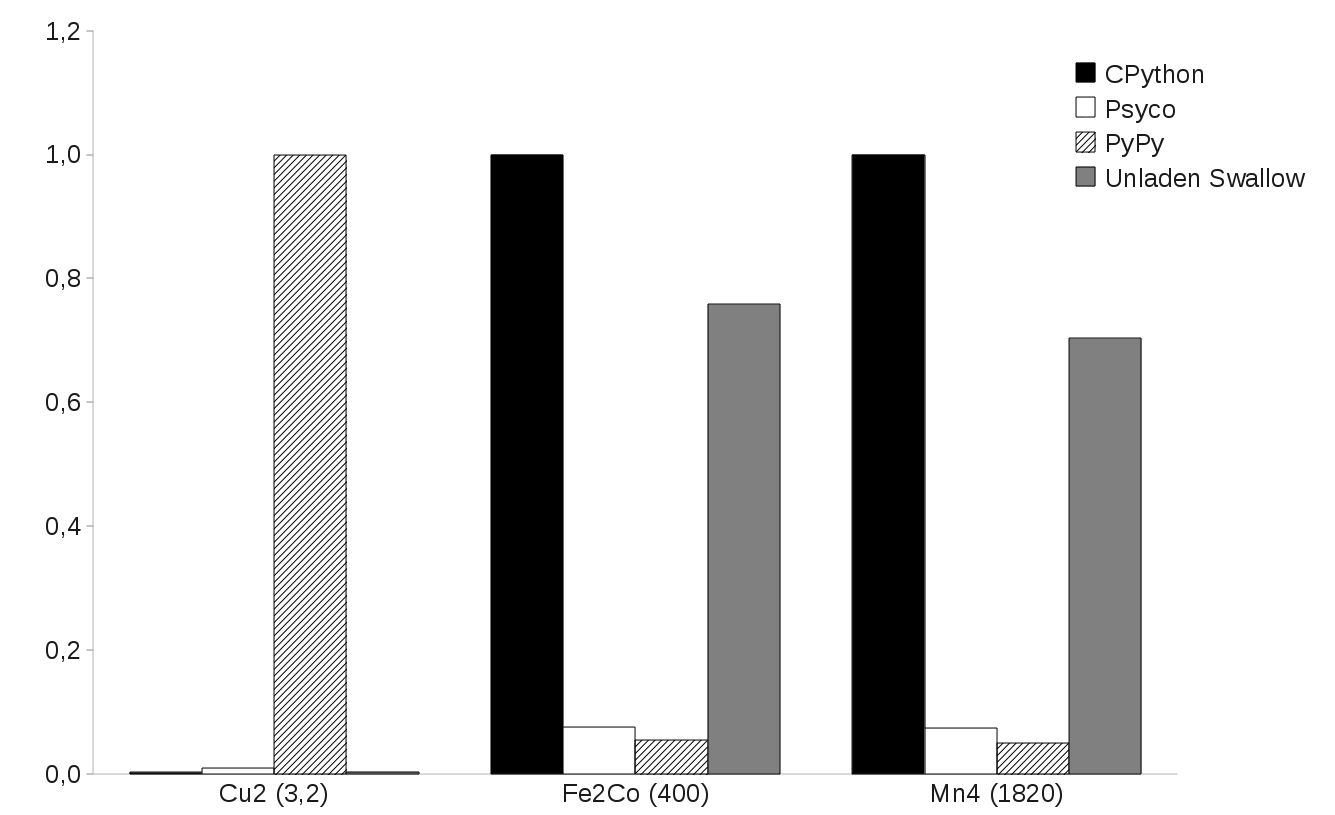
\includegraphics{03_lytvynenko_diagram1.jpg}}
\caption{Дыяграма параўнання адносных часоў выканання праграмы \progname{Mj{\"o}llnir} з рознымі JIT-кампілятарамі (значэнні нармаваныя на час самага павольнага выканання для мадэлі (у дужках, сек)).}
\label{pic:benchmark}
\end{figure}

Такім чынам, для праграмы \progname{Mj{\"o}llnir} найбольш эфектыўным акселератарам выканання на дадзены момант з'яўляецца \progname{PyPy}, і з улікам імклівага развіцця праэкту верагодным ёсць ягонае выкарыстанне ў будучыні як асноўнага (зараз ужываецца \progname{Psyco}). \progname{Psyco} дае блізкія вынікі, \progname{Unladen Swallow} з'яўляецца неэфектыўным. Неадпаведнасць вынікаў для малой мадэлі (Cu\textsubscript{2}), верагодна, абумоўленая затратамі часу на JIT-кампіляцыю, якія не кампенсуюцца праз вельмі малы аб'ём разлікаў.

\begin{longtable}{|>{\bfseries}c|c|c|c|}
\caption{Час выканання праграмы \progname{Mj{\"o}llnir} з рознымі JIT-кампілятарамі, сек.}\label{tab:benchmark}\\
\hline
Мадэль&Cu\textsubscript{2}&Fe\textsubscript{2}Co&Mn\textsubscript{4}\\
\hline\endfirsthead
\hline
Мадэль&Cu\textsubscript{2}&Fe\textsubscript{2}Co&Mn\textsubscript{4}\\
\hline\endhead
Базісныя функцыі&4&432&625\\
\hline
\progname{CPython 2.6.2}&$0,0075 \pm 0,0002$&$400 \pm 7$&$1820 \pm 20$\\
\hline
\progname{Psyco 1.6}/\progname{CPython 2.6.2}&$0,0304 \pm 0,0002$&$30,5 \pm 0,3$&$134 \pm 1$\\
\hline
\progname{PyPy 1.5} &$3,2 \pm 0,1$&$21,8 \pm 0,6$&$91 \pm 2$\\
\hline
\progname{Unladen Swallow 2009Q3}&$0,010 \pm 0,005$&$303 \pm 4$&$1280 \pm 20$\\
\hline
\end{longtable}

\aknowl{Аўтар дзякуе С.А.Літвіненку за каштоўныя парады пры выкананні гэтае работы.}


\begin{thebibliography}{9}

\bibitem{pDynamo} M. J. Field, The pDynamo Library for Molecular Simulations using Hybrid Quantum Mechanical and Molecular Mechanical Potentials, J. Chem. Theo. Comp.,  4, 2008, 1151--1161.

\bibitem{Mjollnir} А.С. Литвиненко, Е.А. Михалева, С.В.Колотилов, В.В.Павлищук, Влияние спин-орбитального взаимодействия на магнитную восприимчивость полиядерных комплексов 3d-металлов, содержащих ион Co\textsuperscript{2+}, Теорет. и эксперим. химия, 2010, т. 46, с. 403--409.

\bibitem{Optimize} <<Сказ о летающем змее. Агрессивная оптимизация программ на Python'e>>,  http://www.xakep.ru/magazine/xa/123/102/1.asp

\bibitem{speed} <<PyPy Speed Center: Comparison>>, http://speed.pypy.org/comparison/
\end{thebibliography}

\end{document}
